
%(BEGIN_QUESTION)
% Copyright 2007, Tony R. Kuphaldt, released under the Creative Commons Attribution License (v 1.0)
% This means you may do almost anything with this work of mine, so long as you give me proper credit

Sketch wires in this diagram to show how a PLC could be connected to a couple of pressure switches and a motor contactor to control the starting and stopping of a three-phase air compressor motor.  Note that both pressure switches are normally-open: the contacts are open at atmospheric pressure (0 PSIG), and close as pressure rises.  One switch has a setting of 40 PSI, and controls when the motor starts.  The other switch has a setting of 80 PSI, and controls when the motor stops.

$$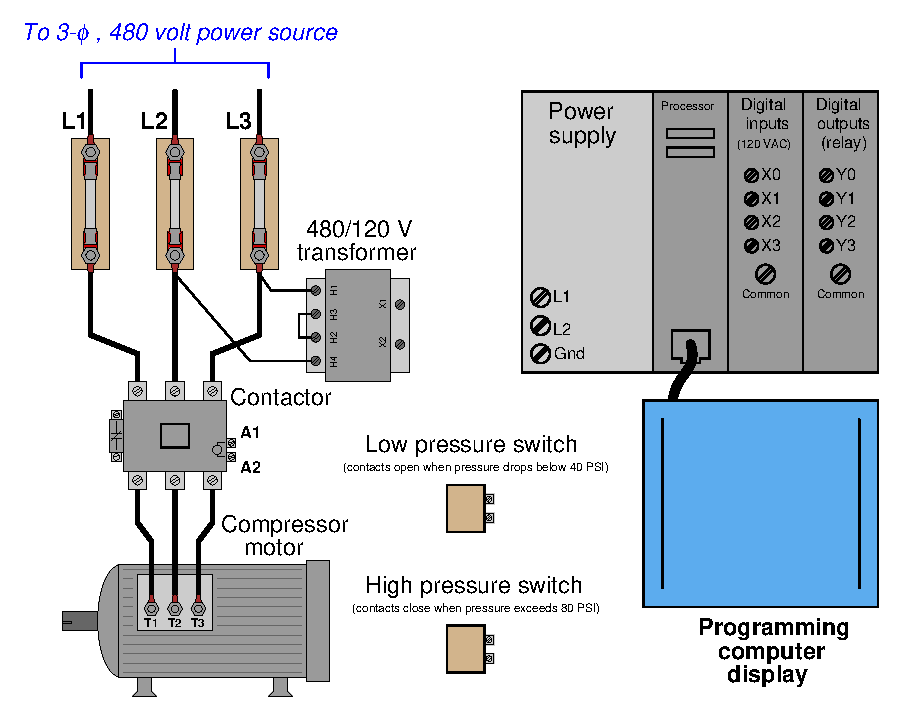
\includegraphics[width=15.5cm]{i02364x01.eps}$$

Also draw a simple ladder logic program in the computer display window for this compressor start/stop function.

\vfil

\underbar{file i02364}
\eject
%(END_QUESTION)





%(BEGIN_ANSWER)

This is a graded question -- no answers or hints given!

%(END_ANSWER)





%(BEGIN_NOTES)

Note how neither pressure switches are form C (having both NO and NC contacts to choose from).  Instead, both pressure switches are form A (normally-open).

\vskip 10pt

Since we need the compressor to turn on when the pressure is less than the low-pressure trip value of 40 PSI, we need the ladder diagram program contacts to both be colored when both pressure switches are open.  This means the virtual contacts must both be drawn as normally-closed (NC).

We have the freedom to choose any of the four available input channels to use for these two pressure switches.  I happen to have used X0 and X1, but I could have just as easily employed X2 and X3, or any other combination of two out of the four channels.  Likewise, any of the four output channels may be used to energize the contactor -- the choice of which particular one to use is arbitrary.  The important detail here is that the channel connected to the low-pressure switch must be the one whose virtual contact in the program is paralleled by a seal-in contact driven by the output bit.

$$\includegraphics[width=15.5cm]{i02364x02.eps}$$

Note that it also would have been appropriate to use a pair of {\it retentive} (latching) coil instructions in this program to achieve the same end without necessitating a ``seal-in'' contact instruction to latch the motor's state.

%INDEX% PLC, wiring: properly connecting input devices to a PLC
%INDEX% PLC, wiring: properly connecting output devices to a PLC

%(END_NOTES)


